\documentclass[a4paper, 11pt]{scrartcl}
\usepackage{a4}


\usepackage[utf8]{inputenc}
\usepackage{dsfont}
\usepackage{amsmath}
\usepackage{graphicx}
\usepackage{here}
\usepackage[section]{placeins}
\usepackage[ngerman]{babel}
\usepackage{caption}
\usepackage{subcaption}
\usepackage[colorlinks, pdfpagelabels, pdfstartview = FitH, bookmarksopen = true, bookmarksnumbered = true, linkcolor = black, plainpages = false, hypertexnames = false, citecolor = black] {hyperref}
\parindent 0pt


\title{Dokumentation der Projektarbeit}
\author{Florian Weber - 44907}
\date{\today}

\begin{document}
\maketitle	%Deckblatt
\newpage

\tableofcontents 	%Inhaltsverzeichnis
\listoffigures		%Bildverzeichnis
\newpage

\section{Vorwort}
Zu Beginn des Projekts war die Carrera Bahn auf dem Stand, dass die Fahrzeuge konventionell sowie automatisiert gesteuert werden konnten. Außerdem war die Rundenzeitmessung und Visualisierung bereits realisiert. Bei der Energieversorgung konnte zwischen Solarstrom und Netzversorgung gewählt werden.
Die Solarstromversorgung wurde pro Bahn durch 2 Solarpanels und einem Tiefsetzsteller mit konstantem Dutycycle hergestellt, die Netzstromversorgung mit einem 15V Schaltnetzteil.

Die Manuelle Steuerung durch den Nutzer wurde realisiert, indem man die klassischen Carrera Drücker, als Variablen Vorwiderstand eingesetzt hat. Im automatisierten Modus musste ein Potentiometer bedient, um die langsame Geschwindigkeit des Autos einzustellen.
In den schnellen Abschnitten der Strecke wurde dieses Poti  durch ein Relais gebrückt und die volle Versorgungsspannung lag an dem Auto an.
\subsection{Probleme der vorhandenen Carrera Bahn und Zielsetzung zur Projektarbeit}
Der im Vorwort grob erwähnte Aufbau der vorhandenen Anlage wies einige Probleme auf:
\begin{itemize}
	\item 1. Solarstromversorgung und Netzversorgung sind nicht chancengleich ausgeführt.(Die Netzversorgung stellt eine stabilisierte Spannungsquelle dar, die Solarstromversorgung allerdings nicht)
	\item 2. Drift der durch den Poti erzeugten Spannung im automatisierten Modus (Temperaturdrift)
	\item 3. Framerate der Visualisierung ist zu gering, sodass diese immer die selbe Zahlensequenz nach dem Komma anzeigt.
	\item Manchmal wird durch einen Aliasingeffekt das Überschreiten eines Sensors in der Bahn nicht erkannt und die Geschwindigkeit wird nicht umgeschalten.
\end{itemize}
Die Oben genannten Probleme sollten durch ein neues Steuer-/Regelkonzept gelöst werden.
\newpage

\section{Funktion - Hardware}
	Im Folgenden wird der grundlegende Aufbau der Carrera Bahn erklärt.

	Diese Beschreibung ist immer nur für Bahn-A, da die
	Bahn-B analog dazu funktioniert. Dazu wird immer wieder auf die Abbildung \ref{img:signalfluss}, sowie auf die \\Abbildung
	\ref{img:carrerakomplett} Bezug genommen.
	\begin{figure}[h]
		\centering
		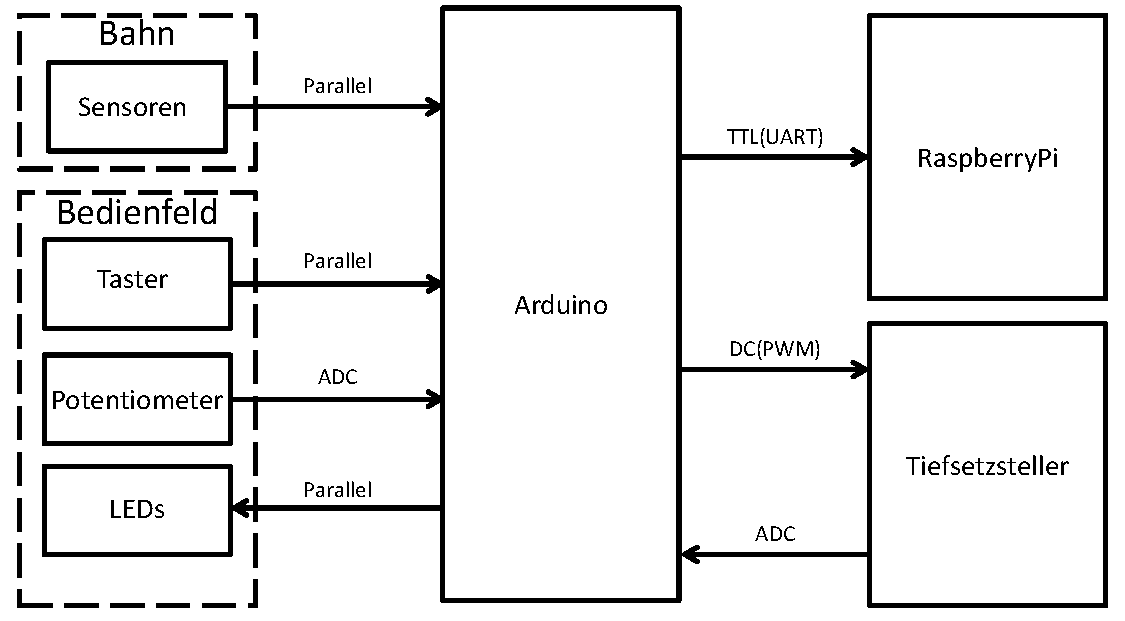
\includegraphics[width=0.85\textwidth]{rec/signalfluss.pdf}
		\caption{Signalfluss}
		\label{img:signalfluss}
	\end{figure}
	\begin{figure}[h]
	\centering
	\includegraphics[width=0.85\textwidth]{rec/Carrerabahnroh.png}
	\caption{Überblick über die Carrera-Bahn}
	\label{img:carrerakomplett}
	\end{figure}
	\newpage

	\subsection{Sensoren}
		Pro Schiene gibt es 3 Sensoren die als Gabellichtschranke ausgeführt sind. Sensor 0 befindet sich am Start, Sensor 1 vor dem Looping und 		Sensor 2 Nach dem Looping.\\

		Sensor 0 wird im Wesentlichen nur zur Zeitmessung genutzt, dazu später mehr.
		Sensor 1 wird genutzt um ein Signal zu generieren, so dass die Steuerung das Auto im Automatik-Modus für den Looping beschleunigen kann. 		Das Signal von Sensor 2 wird schließlich genutzt um nach dem Looping wieder die langsame Geschwindigkeit zu triggern.\\
		Im manuellen Modus dienen die Sensoren nur zur Zeitmessung für die Visualisierung.
		Da die Flanke nur sehr kurz ist, lässt sich diese nicht per Polling ohne Aliasing Effekte digitalisieren. Stattdessen wurden die Hardware 		Pin Change Interrupts des Atmega2560 genutzt.
	\subsection{Bedienschnittstelle}
		\begin{figure}[h]
			\centering
			\includegraphics[width=0.85\textwidth]{rec/hid.png}
			\caption{Bedienschnittstelle}
			\label{img:hid}
		\end{figure}
		Das HID besteht aus 3 Tastern und einem Wechselschalter mit Mittelstellung je Bahn.
		Der Wechselschalter ist zum Auswählen, ob die Bahn mit Energie aus den Solarpanels betrieben wird, oder mit Netzstrom. Ist Dieser in Mittelstellung, wird die Bahn nicht versorgt und das Auto steht - unabhängig des gewählten Modus.
		Über Taster 0 beziehungsweise Taster 1 lässt sich der Modus der Bahn auswählen, welcher durch die LEDs bei den Tastern signalisiert wird. \\Hier steht Automatik und Manuell zur Auswahl.
		Mit Taster 2 lässt sich der Regler der Bahngeschwindigkeit genauer -  Spannung außerhalb des Loopings, auf seinen Startwert zurücksetzen.
	\subsection{Arduino}
		Beim Arduino handelt es sich um einen einfachen Arduino Mega 2560 ADK.\\
		Dieser wurde gewählt da es sich um eine preiswerte Platine handelt, die bereits die wichtigsten Beschaltungen des Mikrocontroller enthält wie zum beispiel die Abblockcondensatoren an der Versorgungsspannung aber auch einen USB-Seriell Wandler den man nutzen kann um sich Daten parallel zum Prozess an ein Terminal auszugeben.
		Letzteres lässt sich sehr gut für das Debugging nutzen.
	\subsection{RaspberryPi}
		Die Visualisierung ist durch ein RaspberryPi Model 3 B realisiert. Dieser empfängt per Uart die codierten Signale der Sensoren, sowie des Reset Tasters der Visualisierung.
		Die Visualisierung war zu Beginn der Projektarbeit bereits vorhanden und in Form eines Python Skripts implementiert.
	\subsection{Tiefsetzsteller}
		Die Tiefsetzsteller fungieren als Stellglieder der Spannungsregelungen der Bahnen.
		Jeder bekommt sein PWM-Signal(Steuergröße) direkt vom Arduino. Desweiteren ist über ein Shunt eine
		Strommessung realisiert. Der Wert liegt zwar im Arduino digital vor, wird allerdings nicht weiter
		verarbeitet und ist lediglich für weiterführende Projekte gedacht. Da die Ausgangsspannung des
		Tiefsetzstellers größer sein kann wie die Referenzspannung des ADC,
		wird diese über einen Spannungsteiler angepasst und auf einen Kanal des ADC geführt.
		Diese Spannung stellt die Regelgröße dar.
	\newpage

\section{Software}
	\subsection{RaspberryPi}

		Bei der Software die auf dem RaspberryPi ausgeführt wird, handelt es sich um ein Python Skript.
		Dieses war zu Beginn der Projektarbeit bereits vorhanden und hat die Sensoren
		der Bahn parallel eingelesen. Mit den Flanken der Sensoren wurde die Rundenzeit gemessen
		und die Bestzeit ermittelt.\\
		Dieses Skript wurde größtenteils übernommen und lediglich in der Richtung abgeändert,
		dass die Trigger-Signale der Sensoren nun über die Serielle Schnittstelle dem Pi mitgeteilt wurden.
		Desweiteren wurden diverse Bugs behoben wie zB die zu geringe Framerate der Visualisierung.
		Als serielle Schnittstelle wurde "ttyAMA0" benutzt.
		\newpage
	\subsection{Arduino}
		Die Software des Arduinos wurde, wie oben bereits erwähnt, nicht in der Arduino Entwicklungsumgebung
		geschrieben. Stattdessen habe ich auf die IDE "AtmelStudio7" zurückgegriffen und den Mikrocontroller
		per ISP beschrieben. Der Bootloader des Arduino musste dazu entfernt werden.
		Gründe dazu waren unter anderem die Wahl der Sprache C++,
		aber auf die Möglichkeit direkt auf die Hardware zuzugreifen(Timer, Hardwareinterrupts...).
		Letzteres ist notwendig um das Timing des Controllers exakt zu steuern.\\
		\subsubsection{Interupts}
		\begin{figure}[h]
			\centering
			\begin{subfigure}{0.47\textwidth}
				\centering
				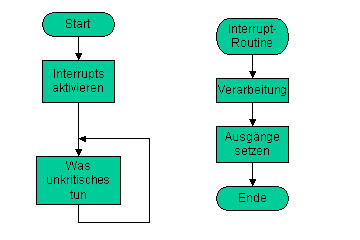
\includegraphics[width=1.1\textwidth]{rec/Interrupt_Programme.png}
				\caption{Interruptgesteuerter \\Programmablauf}
				\label{InterruptgesteuerterProgrammablauf}
			\end{subfigure}
			\begin{subfigure}{0.47\textwidth}
				\centering
				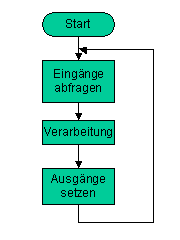
\includegraphics[width=0.55\textwidth]{rec/Sequentielle_Programme.png}
				\caption{Sequentieller \\Programmablauf}
				\label{SequentiellerProgrammablauf}
			\end{subfigure}
			\caption[Möglichkeiten zum Programmablauf]{Möglichkeiten zum Programmablauf
			\\Quelle:Mikrocontroller.net}
			\label{Programmablauf}
		\end{figure}
Der Programmablauf ist größtenteils Interruptgesteuert.
			Dies hat den Vorteil, dass das Timing nichtmehr von der Länge der MainLoop abhängt und Dinge wie zum  Beispiel der Regelagorythmus immer in der selben Frequenz ausgeführt werden.
			Interruptquellen des Programms sind:
			\begin{itemize}
				\item Timer
				\begin{itemize}
					\item[1.] Timer1, Compareregister B match
					\item[2.] Timer3, Compareregister A match
					\item[3.] Timer4, Compareregister A match
				\end{itemize}
				\item Pin Change Interrupts
				\begin{itemize}
					\item[4.] PCINT0\underline{ }vect
					\item[5.] PCINT1\underline{ }vect
					\item[6.] PCINT2\underline{ }vect
				\end{itemize}
			\end{itemize}
			\newpage
			Zu Anfang des Programms wird die ganze Peripherie initialisiert, und die Variablen mit ihren default Werten geladen.
			Anschliesend werden die Interrupts global freigegeben. Ab hier ist die Steuerung Funktionsfähig.
			Wenn ein Auto nun auf, Beispielsweise Sensor 0(Bahn A, am Start), fährt wird der Pegel kurze Zeit \emph{low} und nach verlassen des Sensors wieder \emph{high}.\\ Da Sensor 0 an PCINT16 angeschlossen ist und 16 im Bereich [16,23] liegt, wird das letzte Pin Change Interrupt, PCINT2\underline{ }vect, zweimal ausgelöst. In der ISR (Interrupt Service Routine) muss nun unterschieden werden:
			\begin{itemize}
				\item Durch welchen Pin das Interrupt ausgelöst wurde
				\begin{itemize}
					\item war es ein High $\rightarrow$ Low Übergang
					\item war es ein Low $\rightarrow$ High Übergang
				\end{itemize}
			\end{itemize}
			Zum Entprellen des Eingangs wird direkt, nachdem das Event gehandelt wurde, der Eingang deaktiviert. Danach wird ein Software-Timer gestartet der den Eingang nach dessen Ablauf wieder aktiviert. Mit diesem einfachen Prinzip wird sichergestellt, dass wenn das Auto beim Überahren des Sensors das dementsprechende Event nur einmal triggert.
			Analog zu diesem Sensor 0, ist dies für jeden Sensor sowie Taster realisiert. Die Belegung der benutzten Pin Change Interupts kann Tabelle \ref{tab:belegungpcint} entnommen werden.
			\begin{table}[h]
				\begin{tabular}{|l|l|l|}
					\hline
					Zugehörigkeit & Signal & Bezeichnung\\
					\hline
					\hline
					PCINT0\underline{ }vect & PCINT4 & Button: B-Automatik\\
					\hline
											& PCINT5 & Button: B-Manuell\\
					\hline
											& PCINT6 & Button: A-Automatik\\
					\hline
					\hline
					PCINT1\underline{ }vect & PCINT9 & Button: A-Reset\\
					\hline
											& PCINT10 & Button: B-Reset\\
					\hline
					\hline
					PCINT2\underline{ }vect & PCINT16 & Sensor: 0\\
					\hline
											& PCINT17 & Sensor: 1\\
					\hline
											& PCINT18 & Sensor: 2\\
					\hline
											& PCINT19 & Sensor: 3\\
					\hline
											& PCINT20 & Sensor: 4\\
					\hline
											& PCINT21 & Sensor: 5\\
					\hline
											& PCINT22 & Button: Reset/Shutdown Pi\\
					\hline
											& PCINT23 & Button: A-Manuell\\
					\hline
				\end{tabular}
				\caption{Belegung der Pin Change Interupts}
				\label{tab:belegungpcint}
			\end{table}

	\newpage

\section{Bedienungsanleitung}
		Die Carrera-Bahn beherrscht 2 Modi.
		\begin{itemize}
			\item Manuelles Fahren
			\item Automatisiertes Fahren
		\end{itemize}
		Die Modi können unabhängig voneinander auf beiden Bahnen gewählt werden, sodass man zum Beispiel manuell
		gegen ein Automatisiertes Fahrzeug antreten kann.
		Die Wahl eines dementsprechenden Modus wird durch eine Led über, beziehungsweise unter, des jeweiligen
		Tasters des gewählten Modus signalisiert.
		Außerdem kann die Energieversorgung der Bahn mit dem Wechselschalter ausgewählt werden.
		Unabhängig des gewählten Modus, wird in der Visualisierung die Zeit der 2 Abschnitte, sowie die
		Rundenzeit angezeigt. Nach 30 Runden ist das Rennen vorbei und die Visualisierung wird statisch.
	\subsection{Manuelles Fahren}
		Im Modus Manuelles Fahren kann das Fahrzeug konventionell über die orginalen Carrera Handregler gesteuert
		werden.
	\subsection{Automatisiertes Fahren}
		Der Automatisierte Modus ist aufgeschlüsselt in 2 Zustände:
		\begin{itemize}
			\item Auto-wait
			\item Auto-run
		\end{itemize}
		Immer wenn in den Modus des Automatisierten Fahrens gewechselt wird, startet die Steuerung in
		Auto-wait und das Auto steht.
		Durch kurzes durchdrücken des zugehörigen Handreglers wechselt das Auto in den Auto-run Zustand.
		\subsubsection{Auto-run}
			Im Auto-run Zustand fährt das Auto selbständig. Die Strecke ist in 3 Abschnitte unterteilt.
			\begin{itemize}
				\item{1.} Startlinie $\rightarrow$ Vor dem Looping
				\item{2.} Vor dem Looping $\rightarrow$ Nach dem Looping
				\item{3.} Nach dem Looping $\rightarrow$ Startlinie
			\end{itemize}
			Die Grenze dafür ist durch die Position der Sensoren festgelegt und somit nicht variabel.
			In der Visualisierung ist 1. und 2. in Abschnitt-1 zusammegefasst. \\3. bildet dort Abschnitt-2.
			\newpage

\newpage

\section{Zusammenfassung}
\newpage

\section{Quellenverzeichnis}
\newpage

\section{Anhang}
\subsection{Pinbelegung}
\subsubsection{Arduino}
\subsubsection{RaspberryPi}
\end{document}
